\documentclass[tikz,border=8pt]{standalone}
\usepackage{ctex}
\usepackage{amsmath,amssymb,bm}
\usetikzlibrary{arrows.meta,calc,angles,quotes,patterns,positioning,decorations.pathmorphing}
\definecolor{ink}{RGB}{30,43,58}
\definecolor{blue}{RGB}{37,91,166}
\definecolor{orange}{RGB}{219,113,25}
\definecolor{green}{RGB}{39,139,94}
\definecolor{red}{RGB}{192,52,52}
\tikzset{line cap=round,line join=round,body/.style={draw=ink,very thick},
axis/.style={-{Latex[length=2.5mm]},draw=ink,very thick},
vec/.style={-{Latex[length=2.5mm]},draw=blue,very thick},
force/.style={-{Latex[length=2.5mm]},draw=red,very thick},
guide/.style={draw=ink!45,dashed},dim/.style={{Latex[length=2mm]}-{Latex[length=2mm]},draw=ink!75}}

\usetikzlibrary{decorations.pathmorphing}
\tikzset{mass/.style={circle,draw,fill=white,minimum size=7mm},curve/.style={very thick,blue},rope/.style={very thick,blue},ray/.style={very thick,blue,-{Latex}},impulse/.style={very thick,orange,-{Latex}},resistor/.style={thick,decorate,decoration={zigzag,segment length=3mm,amplitude=1mm}}}
\begin{document}
% 1 question-01
\begin{tikzpicture}[x=1cm,y=1cm,font=\small]

\draw[body,fill=gray!15] (-3,-.2) rectangle (3,0);\node[below] at (0,-.2) {撞击板};
\draw[body,fill=orange!20] (-.45,1.9) rectangle (.45,2.8);\draw[vec] (0,1.8)--(0,1) node[right] {$v_0$};
\foreach \x in {-2,-1,1,2}{\draw[vec] (\x,.3)--(\x,1.5);}\node[blue] at (-2.8,1.7) {反向空气};
\draw[guide] (-3,3.3)--(3,3.3);\draw[dim] (3.5,0)--(3.5,3.3) node[midway,right] {$h_0$};\node at (0,4) {颗粒仍在空气层内时受到阻力；图为竖直截面};

\end{tikzpicture}

% 2 solution-01
\begin{tikzpicture}[x=1cm,y=1cm,font=\small]

\draw[body] (-1,-1)--(5,-1);\draw[body,fill=orange!20] (-.4,1) rectangle (.4,1.8);\draw[body,fill=orange!20] (3,1.4) circle(.4);
\draw[force] (0,1.4)--(0,2.8) node[above] {$F_{\rm cyl}$};\draw[vec] (.6,1.4)--(.6,.2) node[below] {$v$};\draw[force] (3,1.4)--(3,2.8) node[above] {$F_{\rm sph}$};
\node[align=left,anchor=west] at (5.8,1.4) {相对速度 $U=v_0+v$ 随颗粒减速而改变\\[6pt]$v\,dv/dz=-\eta\rho_0(v_0+v)^2/(\rho r)$\\[6pt]$s=\rho r(\ln2-1/2)/(\eta\rho_0)$\\[6pt]恒定 $U=2v_0$ 另列为初值估算};

\end{tikzpicture}

% 3 question-02
\begin{tikzpicture}[x=1cm,y=1cm,font=\small]
\draw[body] (-3,0) arc(180:360:3);\fill (0,0) circle(2pt) node[above] {$O$};
\draw[orange,ultra thick] (-0.014078,-2.999967)--(1.705528,-2.468031);
\fill (-0.014078,-2.999967) circle(2pt) node[left] {$A$};
\fill (1.705528,-2.468031) circle(2pt) node[right] {$B$};
\fill (0.845725,-2.733999) circle(2pt) node[below] {$G$};
\draw[guide] (0.000000,0.000000)--(0.845725,-2.733999);
\node[align=left,anchor=west] at (4.3,-1.1) {$R>1.5L$\\[6pt]均匀杆长为 $L$\\[6pt]两端均接触圆周，杆与 $OG$ 垂直};
\end{tikzpicture}

% 4 solution-02
\begin{tikzpicture}[x=1cm,y=1cm,font=\small]
\draw[body] (-3,0) arc(180:360:3);\fill (0,0) circle(2pt) node[above] {$O$};
\draw[orange,ultra thick] (-0.014078,-2.999967)--(1.705528,-2.468031);
\fill (-0.014078,-2.999967) circle(2pt) node[left] {$A$};
\fill (1.705528,-2.468031) circle(2pt) node[right] {$B$};
\fill (0.845725,-2.733999) circle(2pt) node[below] {$G$};
\draw[guide] (0.000000,0.000000)--(0.845725,-2.733999);
\node[align=left,anchor=west] at (4.3,-1.1) {$d=\sqrt{R^2-L^2/4}$\\[6pt]$K=d^2+L^2/12$\\[6pt]两端均接触圆周，杆与 $OG$ 垂直};\draw[force] (-0.014078,-2.999967)--(-0.009151,-1.949979);
\draw[force] (1.705528,-2.468031)--(1.108593,-1.604220);
\draw[force] (0.845725,-2.733999)--(0.845725,-3.733999);
\node[right] at (1.1,-3.8) {$mg$};
\end{tikzpicture}

% 5 question-03
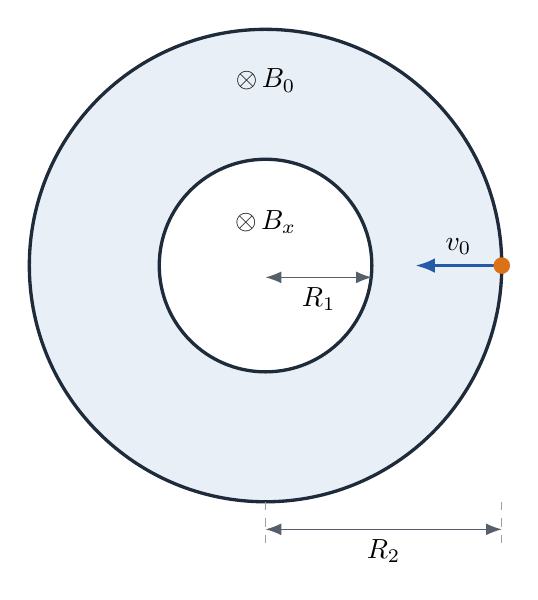
\begin{tikzpicture}[scale=1]
  \fill[blue!10] (0,0) circle(3);
  \fill[white] (0,0) circle(1.35);
  \draw[body] (0,0) circle(3) (0,0) circle(1.35);
  \node at (0,2.35) {$\otimes\,B_0$};
  \node at (0,.55) {$\otimes\,B_x$};
  \draw[vec] (3,0)--(1.9,0) node[midway,above] {$v_0$};
  \fill[orange] (3,0) circle(3pt);
  \draw[dim] (0,-.15)--(1.35,-.15) node[midway,below] {$R_1$};
  \draw[dim] (0,-3.35)--(3,-3.35) node[midway,below] {$R_2$};
  \draw[guide] (0,-3)--(0,-3.6) (3,-3)--(3,-3.6);
\end{tikzpicture}

% 6 solution-03
\begin{tikzpicture}[x=1cm,y=1cm,font=\small]
\draw[body] (0,0) circle(2);\draw[body] (0,0) circle(.9);\draw[vec] (3.2,0)--(2,0) node[midway,above] {$v_{0,\rm crit}$};
\draw[orange,very thick] plot coordinates {(2.000000,0.000000) (1.987405,-0.000045) (1.974811,-0.000179) (1.962218,-0.000403) (1.949628,-0.000716) (1.937039,-0.001119) (1.924454,-0.001611) (1.911873,-0.002193) (1.899296,-0.002864) (1.886724,-0.003624) (1.874158,-0.004474) (1.861598,-0.005413) (1.849045,-0.006441) (1.836500,-0.007558) (1.823963,-0.008765) (1.811435,-0.010060) (1.798917,-0.011445) (1.786409,-0.012918) (1.773911,-0.014481) (1.761425,-0.016132) (1.748951,-0.017872) (1.736490,-0.019700) (1.724042,-0.021617) (1.711608,-0.023622) (1.699188,-0.025716) (1.686784,-0.027898) (1.674395,-0.030168) (1.662023,-0.032526) (1.649668,-0.034972) (1.637331,-0.037505) (1.625012,-0.040127) (1.612712,-0.042835) (1.600431,-0.045631) (1.588171,-0.048514) (1.575931,-0.051485) (1.563713,-0.054542) (1.551517,-0.057686) (1.539344,-0.060916) (1.527194,-0.064233) (1.515067,-0.067637) (1.502966,-0.071126) (1.490889,-0.074701) (1.478838,-0.078362) (1.466813,-0.082109) (1.454816,-0.085941) (1.442845,-0.089858) (1.430903,-0.093860) (1.418990,-0.097947) (1.407106,-0.102118) (1.395252,-0.106374) (1.383429,-0.110713) (1.371636,-0.115137) (1.359876,-0.119645) (1.348147,-0.124236) (1.336452,-0.128910) (1.324790,-0.133667) (1.313163,-0.138507) (1.301570,-0.143429) (1.290012,-0.148434) (1.278490,-0.153521) (1.267004,-0.158689) (1.255556,-0.163939) (1.244145,-0.169270) (1.232773,-0.174682) (1.221439,-0.180175) (1.210144,-0.185748) (1.198889,-0.191402) (1.187675,-0.197135) (1.176502,-0.202948) (1.165370,-0.208840) (1.154281,-0.214811) (1.143234,-0.220860) (1.132231,-0.226988) (1.121271,-0.233194) (1.110356,-0.239478) (1.099485,-0.245839) (1.088661,-0.252277) (1.077882,-0.258793) (1.067149,-0.265384) (1.056464,-0.272052) (1.045827,-0.278795) (1.035238,-0.285614) (1.024697,-0.292507) (1.014206,-0.299476) (1.003764,-0.306519) (0.993373,-0.313636) (0.983033,-0.320827) (0.972744,-0.328091) (0.962507,-0.335428) (0.952322,-0.342837) (0.942190,-0.350319) (0.932112,-0.357872) (0.922087,-0.365497) (0.912117,-0.373193) (0.902202,-0.380960) (0.892343,-0.388797) (0.882539,-0.396703) (0.872792,-0.404680) (0.863101,-0.412725) (0.853469,-0.420839) (0.843894,-0.429021) (0.834377,-0.437271) (0.824919,-0.445589) (0.815521,-0.453973) (0.806182,-0.462424) (0.796904,-0.470941) (0.787687,-0.479524) (0.778530,-0.488172) (0.769436,-0.496886) (0.760404,-0.505663) (0.751434,-0.514504) (0.742527,-0.523409) (0.733684,-0.532378) (0.724905,-0.541408) (0.716190,-0.550501) (0.707540,-0.559656) (0.698955,-0.568871) (0.690436,-0.578148) (0.681983,-0.587485) (0.673597,-0.596881)};
\fill (0.673597,-0.596881) circle(2pt) node[left] {$Q$};
\fill (2.000000,-1.772222) circle(2pt) node[below] {$C_\rho$};
\draw[guide] (0.000000,0.000000)--(2.000000,-1.772222);
\draw[guide] (0.673597,-0.596881)--(2.000000,-1.772222);
\node[align=left,anchor=west] at (4.7,-.1) {$\rho=(R_2^2-R_1^2)/(2R_1)$\\[6pt]$|OC_\rho|=R_1+\rho$\\[6pt]临界轨道在 $Q$ 与内圆相切\\[6pt]真正进入内圆须 $v_0>v_{0,\rm crit}$};
\end{tikzpicture}

% 7 question-04
\begin{tikzpicture}[x=1cm,y=1cm,font=\small]

\draw[body] (-3,0)--(0.8944271909999159,0)--(0.8944271909999159,0.4)--(3,0.4);\draw[body] (0,1.2) circle(1.2);\fill (0,1.2) circle(2pt) node[above] {$O$};\fill (0.8944271909999159,0.4) circle(2pt) node[right] {$A$};
\draw[dim] (0,1.2)--(0.8944271909999159,0.4) node[midway,above] {$r$};\draw[dim] (2.8,0)--(2.8,0.4) node[midway,right] {$h$};\draw[vec] (-2,1.2)--(-.5,1.2) node[above] {$v_0$};
\node[align=left,anchor=west] at (4,1) {碰撞后绕台阶角 $A$ 转动\\碰前圆环向右纯滚动\\越障条件与停止时间待求};

\end{tikzpicture}

% 8 solution-04
\begin{tikzpicture}[x=1cm,y=1cm,font=\small]

\draw[body] (-2,0)--(2,0);\draw[body] (0,1) circle(1);\fill (0,1) circle(2pt) node[left] {$O$};
\draw[force] (0,1)--(0,.1) node[left] {$mg$};\draw[force] (0,0)--(0,.8) node[right] {$N$};\draw[force] (0,0)--(-1,0) node[below] {$f$};
\coordinate (P) at (-.707,1.707);\draw[force] (-1.7,2.7)--(P) node[midway,left] {$P_n$};\draw[force] (P)--(.1,2.5) node[above] {$\mu P_n$};
\draw[orange,very thick,-{Latex}] (1.3,.7) arc(-30:30:1.5) node[right] {$kN$};
\node[align=left,anchor=west] at (4,1.2) {受力点区分：重力在 $O$，摩擦在接触点\\[6pt]棍的法向与切向力互相垂直\\[6pt]滚动阻力偶矩与滚动角速度反向};

\end{tikzpicture}

% 9 question-05
\begin{tikzpicture}[x=1cm,y=1cm,font=\small]

\foreach \x/\w/\lab in {0/1/1,2/2/2,5/1/3}{\draw[body] (\x,3.3)--(\x,0)--(\x+\w,0)--(\x+\w,3.3);\node at (\x+\w/2,3.7) {$S_{\lab}$};}
\draw[blue,thick] (0,2.4)--(1,2.4);\draw[blue,thick] (2,2.4)--(4,2.4);\draw[blue,thick] (5,.8)--(6,.8);
\draw[guide] (-.3,2)--(6.3,2) node[right] {平衡液面};\draw[dim] (.5,2)--(.5,2.4) node[right] {$l\epsilon$};\draw[dim] (5.5,.8)--(5.5,2) node[right] {$3l\epsilon$};
\draw[body] (1,.3)--(2,.3);\draw[body] (4,.3)--(5,.3);\node[align=center] at (3,-.8) {$S_1:S_2:S_3=1:2:1$；位移定义为 $lx_i$};

\end{tikzpicture}

% 10 solution-05
\begin{tikzpicture}[x=1cm,y=1cm,font=\small]

\draw[axis] (0,0)--(6.5,0) node[right] {$t\sqrt{g/l}$};\draw[axis] (0,-3.4)--(0,1.6) node[above] {$x_i/\epsilon$};
\draw[blue,very thick,domain=0:6.28,samples=100] plot(\x,{cos(\x r)});\draw[orange,very thick,domain=0:6.28,samples=100] plot(\x,{-3*cos(\x r)});
\node[blue] at (3.14,1.5) {$x_1=x_2=\epsilon\cos\omega t$};\node[orange] at (3.14,-3.6) {$x_3=-3\epsilon\cos\omega t$};\node at (3,3.8) {$\omega=\sqrt{g/l}$；两条曲线按振幅比例绘制};

\end{tikzpicture}

% 11 question-06
\begin{tikzpicture}[x=1cm,y=1cm,font=\small]

\draw[body] (0,1.4)--(6,1.4)--(6,-1.4)--(0,-1.4);\node[left] at (0,0) {左端出口};\node[right] at (6,0) {保留右壁};
\foreach \x/\y/\s in {1/.6/1,2/-.5/-1,3/.4/1,4/-.7/-1,5/.6/1}{\fill (\x,\y) circle(2pt);\draw[vec] (\x,\y)--(\x+.6*\s,\y+.2);}
\draw[dim] (0,-2)--(6,-2) node[midway,below] {$l$};\node at (3,2) {初始热平衡：分子速度既有向右也有向左};

\end{tikzpicture}

% 12 solution-06
\begin{tikzpicture}[x=1cm,y=1cm,font=\small]
\draw[axis] (0,0)--(4.4,0) node[right] {$v_x$};\draw[axis] (0,0)--(0,2.1) node[above] {$f(v_x)$};\fill[blue!15] (1.2,0)--plot[domain=1.2:4,samples=100](\x,{1.8*exp(-\x*\x/2)})--(4,0)--cycle;\draw[blue,very thick,domain=0:4,samples=100] plot(\x,{1.8*exp(-\x*\x/2)});\draw[guide] (1.2,0)--(1.2,1.2);\node[below] at (1.2,0) {$(l-x)/t$};\node[align=left,anchor=west] at (5,1.2) {位置为 $x$、初速度向右的分子\\[6pt]撞右壁须 $v_x>(l-x)/t$\\[6pt]初速度向左者直接逸出，不撞右壁\\[6pt]撞壁计数与冲量使用不同积分权重};
\end{tikzpicture}

% 13 question-07
\begin{tikzpicture}[scale=1]
  \draw[axis] (-5,0)--(5,0);
  \draw[body] (-3.8,-1.5)--(-3.8,1.5) node[above] {物屏};
  \draw[blue,very thick] (0,-1.5) arc[start angle=-90,end angle=90,x radius=.25,y radius=1.5];
  \draw[blue,very thick] (3,-1.25) arc[start angle=-90,end angle=90,x radius=.22,y radius=1.25];
  \node at (0,-1.85) {$L_1,D_1$}; \node at (3,-1.6) {$L_2,D_2$};
  \draw[dim] (-3.8,2)--(0,2) node[midway,above] {$l_1$};
  \draw[dim] (0,2)--(3,2) node[midway,above] {$l_2$};
  \draw[body] (-3.8,0)--(-3.8,1.0);
\end{tikzpicture}

% 14 solution-07
\begin{tikzpicture}[x=1cm,y=1cm,font=\small]

\begin{scope}
\draw[axis] (0,0)--(10,0);\draw[body] (0,-2.8)--(0,2.8) node[above] {物屏};\draw[body] (6,-1.5)--(6,1.5) node[above] {$L_1$};\draw[body] (9,-.5)--(9,.5) node[above] {$L_2$};
\draw[ray] (0,2.5)--(6,-1.5)--(9,-.5)--(10,1/3);\fill (0,2.5) circle(2pt) node[left] {$5D_2/2$};\node[align=center] at (5,-3.5) {极限可见光线：$y_1=-3D_2/2,\ y_2=-D_2/2$\\存在任意一条可通过的光线};
\end{scope}
\begin{scope}[yshift=-9cm]
\draw[axis] (0,0)--(10,0);\draw[body] (0,-1.8)--(0,1.8) node[above] {物屏};\draw[body] (6,-1.5)--(6,1.5) node[above] {$L_1$};\draw[body] (9,-.5)--(9,.5) node[above] {$L_2$};
\draw[ray,orange] (0,1)--(6,0)--(9,-.5)--(10,-1/6);\fill (0,1) circle(2pt) node[left] {$D_2$};\node[align=center] at (5,-2.5) {指定中心光线：$y_1=0,\ y_2=-D_2/2$\\$x$ 按 $f_2$、$y$ 按 $D_2$ 归一化，纵横比例不同};
\end{scope}

\end{tikzpicture}

% 15 question-08
\begin{tikzpicture}[x=1cm,y=1cm,font=\small]
\draw[axis] (0,0)--(2.6,0) node[right] {$ax/c^2$};\draw[axis] (0,0)--(0,4.4) node[above] {$at/c$};\draw[blue,very thick,domain=0:.999,samples=120] plot({2*\x*\x},{4*\x});\draw[orange,very thick,domain=0:.999,samples=120] plot({.4+2*\x*\x},{4*\x});\draw[guide] (0,4)--(2.6,4);\node[left] at (0,4) {$1$};\node[align=left,anchor=west] at (3.4,2) {两端始终具有相同的地面坐标加速度\\蓝：左端，橙：右端\\只定义 $at/c<1$ 的世界线};
\end{tikzpicture}

% 16 solution-08
\begin{tikzpicture}[x=1cm,y=1cm,font=\small]
\draw[axis] (0,0)--(2.6,0) node[right] {$ax/c^2$};\draw[axis] (0,0)--(0,4.4) node[above] {$at/c$};
\draw[blue,very thick] plot coordinates {(0.000000,0.000000) (0.000141,0.033580) (0.000564,0.067160) (0.001269,0.100739) (0.002255,0.134319) (0.003524,0.167899) (0.005074,0.201479) (0.006907,0.235059) (0.009021,0.268639) (0.011417,0.302218) (0.014095,0.335798) (0.017055,0.369378) (0.020297,0.402958) (0.023821,0.436538) (0.027626,0.470118) (0.031714,0.503697) (0.036083,0.537277) (0.040735,0.570857) (0.045668,0.604437) (0.050883,0.638017) (0.056380,0.671597) (0.062159,0.705176) (0.068220,0.738756) (0.074563,0.772336) (0.081188,0.805916) (0.088094,0.839496) (0.095283,0.873076) (0.102753,0.906655) (0.110505,0.940235) (0.118539,0.973815) (0.126856,1.007395) (0.135454,1.040975) (0.144333,1.074555) (0.153495,1.108134) (0.162939,1.141714) (0.172665,1.175294) (0.182672,1.208874) (0.192961,1.242454) (0.203533,1.276034) (0.214386,1.309613) (0.225521,1.343193) (0.236938,1.376773) (0.248637,1.410353) (0.260618,1.443933) (0.272880,1.477513) (0.285425,1.511092) (0.298252,1.544672) (0.311360,1.578252) (0.324750,1.611832) (0.338422,1.645412) (0.352377,1.678992) (0.366613,1.712571) (0.381131,1.746151) (0.395930,1.779731) (0.411012,1.813311) (0.426376,1.846891) (0.442021,1.880471) (0.457949,1.914050) (0.474158,1.947630) (0.490649,1.981210) (0.507422,2.014790) (0.524477,2.048370) (0.541814,2.081950) (0.559433,2.115529) (0.577334,2.149109) (0.595516,2.182689) (0.613981,2.216269) (0.632727,2.249849) (0.651756,2.283429) (0.671066,2.317008) (0.690658,2.350588) (0.710532,2.384168) (0.730688,2.417748) (0.751126,2.451328) (0.771846,2.484908) (0.792847,2.518487) (0.814131,2.552067) (0.835696,2.585647) (0.857544,2.619227) (0.879673,2.652807) (0.902084,2.686387) (0.924777,2.719966) (0.947752,2.753546) (0.971009,2.787126) (0.994548,2.820706) (1.018368,2.854286) (1.042471,2.887866) (1.066855,2.921445) (1.091522,2.955025) (1.116470,2.988605) (1.141700,3.022185) (1.167212,3.055765) (1.193006,3.089345) (1.219082,3.122924) (1.245440,3.156504) (1.272080,3.190084) (1.299001,3.223664) (1.326205,3.257244) (1.353690,3.290824) (1.381457,3.324403) (1.409506,3.357983) (1.437837,3.391563) (1.466450,3.425143) (1.495345,3.458723) (1.524522,3.492303) (1.553981,3.525882) (1.583721,3.559462) (1.613744,3.593042) (1.644048,3.626622) (1.674635,3.660202) (1.705503,3.693782) (1.736653,3.727361) (1.768085,3.760941) (1.799799,3.794521) (1.831795,3.828101) (1.864072,3.861681) (1.896632,3.895261) (1.929473,3.928840) (1.962597,3.962420) (1.996002,3.996000)};
\draw[orange,very thick] plot coordinates {(0.400000,0.000000) (0.400141,0.033580) (0.400564,0.067160) (0.401269,0.100739) (0.402255,0.134319) (0.403524,0.167899) (0.405074,0.201479) (0.406907,0.235059) (0.409021,0.268639) (0.411417,0.302218) (0.414095,0.335798) (0.417055,0.369378) (0.420297,0.402958) (0.423821,0.436538) (0.427626,0.470118) (0.431714,0.503697) (0.436083,0.537277) (0.440735,0.570857) (0.445668,0.604437) (0.450883,0.638017) (0.456380,0.671597) (0.462159,0.705176) (0.468220,0.738756) (0.474563,0.772336) (0.481188,0.805916) (0.488094,0.839496) (0.495283,0.873076) (0.502753,0.906655) (0.510505,0.940235) (0.518539,0.973815) (0.526856,1.007395) (0.535454,1.040975) (0.544333,1.074555) (0.553495,1.108134) (0.562939,1.141714) (0.572665,1.175294) (0.582672,1.208874) (0.592961,1.242454) (0.603533,1.276034) (0.614386,1.309613) (0.625521,1.343193) (0.636938,1.376773) (0.648637,1.410353) (0.660618,1.443933) (0.672880,1.477513) (0.685425,1.511092) (0.698252,1.544672) (0.711360,1.578252) (0.724750,1.611832) (0.738422,1.645412) (0.752377,1.678992) (0.766613,1.712571) (0.781131,1.746151) (0.795930,1.779731) (0.811012,1.813311) (0.826376,1.846891) (0.842021,1.880471) (0.857949,1.914050) (0.874158,1.947630) (0.890649,1.981210) (0.907422,2.014790) (0.924477,2.048370) (0.941814,2.081950) (0.959433,2.115529) (0.977334,2.149109) (0.995516,2.182689) (1.013981,2.216269) (1.032727,2.249849) (1.051756,2.283429) (1.071066,2.317008) (1.090658,2.350588) (1.110532,2.384168) (1.130688,2.417748) (1.151126,2.451328) (1.171846,2.484908) (1.192847,2.518487) (1.214131,2.552067) (1.235696,2.585647) (1.257544,2.619227) (1.279673,2.652807) (1.302084,2.686387) (1.324777,2.719966) (1.347752,2.753546) (1.371009,2.787126) (1.394548,2.820706) (1.418368,2.854286) (1.442471,2.887866) (1.466855,2.921445) (1.491522,2.955025) (1.516470,2.988605) (1.541700,3.022185) (1.567212,3.055765) (1.593006,3.089345) (1.619082,3.122924) (1.645440,3.156504) (1.672080,3.190084) (1.699001,3.223664) (1.726205,3.257244) (1.753690,3.290824) (1.781457,3.324403) (1.809506,3.357983) (1.837837,3.391563) (1.866450,3.425143) (1.895345,3.458723) (1.924522,3.492303) (1.953981,3.525882) (1.983721,3.559462) (2.013744,3.593042) (2.044048,3.626622) (2.074635,3.660202) (2.105503,3.693782) (2.136653,3.727361) (2.168085,3.760941) (2.199799,3.794521) (2.231795,3.828101) (2.264072,3.861681) (2.296632,3.895261) (2.329473,3.928840) (2.362597,3.962420) (2.396002,3.996000)};
\fill (0.500000,2.000000) circle(2pt) node[left] {$A$};
\fill (1.045743,2.272872) circle(2pt) node[right] {$B$};
\draw[green,very thick] (0.500000,2.000000)--(1.045743,2.272872);
\draw[guide] (0,4)--(2.6,4);\node[left] at (0,4) {$1$};\node[align=left,anchor=west] at (3.6,2) {蓝、橙：左、右端世界线\\[6pt]绿色：事件 $A$ 的瞬时同时线\\[6pt]示例 $al/c^2=0.1,\ at_A/c=0.5$\\[6pt]两事件均须满足 $at/c<1$};
\end{tikzpicture}
\end{document}
